\section{Comparable development cross-validation and model selection}
Table~\ref{tab:cv} summarizes the required prevalence baseline, regularized logistic regression, and the target-specific tree model ultimately frozen in T06. Values are Stage~6 common-fold means and sample standard deviations on development data. They are not held-out test results and are descriptive rather than significance tests. The full seven-model comparison is in \texttt{stage6\_catboost\_outputs/stage6\_report.md}; Figure~\ref{fig:cv} shows that broader comparison.

\begin{table}[H]
\centering\small
\caption{Comparable development CV results (mean $\pm$ sample SD, five folds).}\label{tab:cv}
\begin{tabular}{llrrr}\toprule
Target & Model & AP & AUROC & Brier\\\midrule
Death & Dummy prior & $0.160\pm0.002$ & $0.500\pm0.000$ & $0.134\pm0.001$\\
Death & Logistic regression & $0.651\pm0.031$ & $0.879\pm0.017$ & $0.089\pm0.005$\\
Death & CatBoost tuned & $0.733\pm0.059$ & $0.901\pm0.022$ & $0.077\pm0.009$\\\midrule
ZSN & Dummy prior & $0.225\pm0.002$ & $0.500\pm0.000$ & $0.174\pm0.001$\\
ZSN & Logistic regression & $0.315\pm0.030$ & $0.621\pm0.025$ & $0.179\pm0.005$\\
ZSN & Random Forest tuned & $0.502\pm0.083$ & $0.718\pm0.045$ & $0.148\pm0.013$\\\midrule
FIBR\_PREDS & Dummy prior & $0.099\pm0.000$ & $0.500\pm0.000$ & $0.089\pm0.000$\\
FIBR\_PREDS & Logistic regression & $0.246\pm0.068$ & $0.702\pm0.071$ & $0.089\pm0.008$\\
FIBR\_PREDS & Random Forest preliminary & $0.301\pm0.108$ & $0.725\pm0.063$ & $0.083\pm0.005$\\\bottomrule
\end{tabular}
\end{table}
\begin{figure}[H]\centering
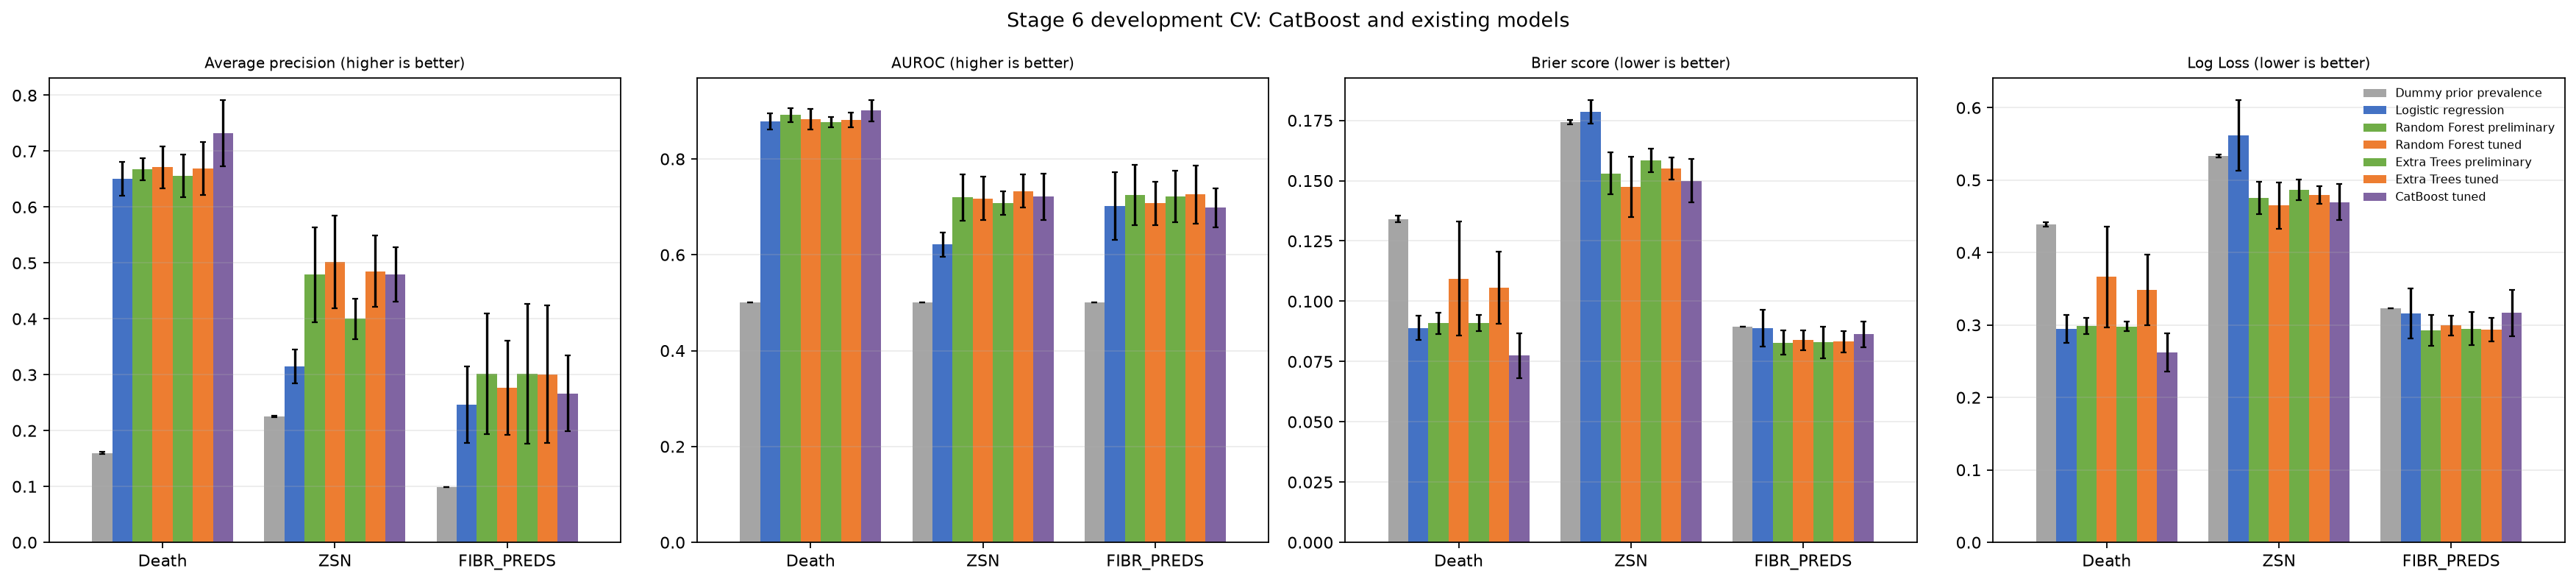
\includegraphics[width=.98\linewidth]{model_comparison.png}
\caption{Stage~6 common-fold comparison across the existing model candidates. Source: \texttt{stage6\_catboost\_outputs/model\_comparison.png}.}\label{fig:cv}
\end{figure}

T06 froze CatBoost tuned for mortality, tuned Random Forest for ZSN, and preliminary Random Forest for fibrillation. Mortality CatBoost had the strongest saved mean AP among the compared candidates (0.7326 versus 0.6713 for tuned RF) and better mean AUROC/Brier evidence. For ZSN, tuned RF had the strongest saved AP (0.5018); Extra Trees tuned was the nearest alternative at 0.4850. For FIBR\_PREDS, preliminary RF and Extra Trees were effectively tied in AP (0.301054 versus 0.301365, gap 0.000311, smaller than either fold SD); RF was retained as a balanced choice because its saved mean AUROC was slightly higher and its Brier/log loss slightly lower. The final manifest identifies these as revision \texttt{non\_tabpfn\_v1}. This selection did not use test outcomes.
